\documentclass[11pt,a4paper]{article}
\usepackage[utf8]{inputenc}
\usepackage{color}
\usepackage{enumerate}
\usepackage{fancyhdr}
\usepackage{minted}
\usepackage{graphicx}
\usepackage{array}
\usepackage{hyperref}
\usepackage[spanish]{babel}

\setlength{\oddsidemargin}{18pt}
\setlength{\headheight}{14pt}
\setlength{\textheight}{609pt}
\setlength{\marginparsep}{11pt}
\setlength{\footskip}{30pt}
\hoffset = 0pt
\voffset = 0pt
\setlength{\topmargin}{0pt}
\setlength{\headsep}{25pt}
\setlength{\textwidth}{424pt}
\setlength{\marginparwidth}{54pt}
\setlength{\marginparpush}{5pt}
\paperwidth = 597pt
\paperheight = 845pt

\pagestyle{fancy}
\fancyhead[LO]{\textcolor[rgb]{0,0,0}{Grado en Ingeniería Informática}}
\fancyhead[RO]{\textcolor[rgb]{0.2,0.2,0.9}{Algorítmica, Curso 2015-2016}}

\hypersetup{
	colorlinks,
	citecolor=black,
	filecolor=black,
	linkcolor=black,
	urlcolor=black
}

\begin{document}

	\begin{titlepage}

		\centering

		\begin{figure}[h]

			\centering
			
\includegraphics[width=0.6\textwidth]{logo-ugr.png}
			
		\end{figure}

		\vspace{1cm}

		{\scshape\LARGE Universidad de Granada}

		\vspace{1cm}

		{\LARGE Algorítmica}

		\vspace{1cm}

		{\huge\bfseries\textit{Análisis de eficiencia algorítmica}}

		\vspace{1cm}

		{\itshape\large 
		Laura Calle Caraballo \\
		Cristina María Garrido López \\
		Germán González Almagro \\
		Javier León Palomares \\
		Antonio Manuel Milán Jiménez}

		\vfill

		{\Large 14 de marzo de 2016}

	\end{titlepage}

\newpage

	\tableofcontents

\newpage

	\section{Introducción.}

		\par
		En este documento se analiza y compara la eficiencia de ocho algoritmos diferentes. Seis de ellos abordan la ordenación de vectores; por otra parte, el algoritmo de Floyd trata la búsqueda del camino más corto entre todos los pares de nodos de un grafo dirigido cualquiera y el algoritmo restante resuelve el problema de las torres de Hanoi.

	\section{Algoritmos de ordenación.}

		\subsection{Algoritmos de orden O($n^2$).}

			\par
			En esta sección, analizaremos la eficiencia empírica e híbrida de los algoritmos Burbuja, Inserción y Selección.

			\par
			Para los cálculos de eficiencia híbrida emplearemos la función: $ax^2+bx+c$.

			\subsubsection{Algoritmo \textit{Burbuja}.}

				\par
				A continuación se muestra la gráfica de tiempos de ejecución obtenida:

				\begin{figure}[h]

					\centering
					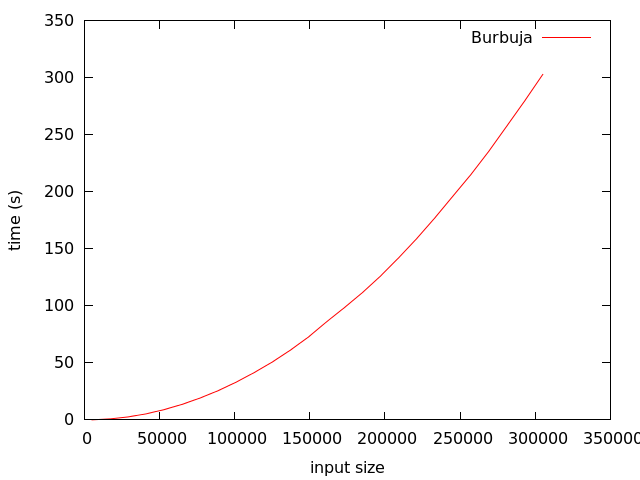
\includegraphics[width=1\textwidth]{burbuja.png}
					\caption{Gráfica del algoritmo \textit{Burbuja}. Compilación sin optimización. Intel® Core™ i7-5500U CPU @ 2.40GHz.}

				\end{figure}

\newpage

				\par
				El análisis híbrido realizado a partir de los datos representados en la gráfica tiene los siguientes resultados:

				\begin{itemize}

					\item
					$a$ $=$ $3.25807\cdot 10^{-9}$
					\item
					$b$ $=$ $-6.62085\cdot 10^{-7}$
					\item
					$c$ $=$ $0.0683299$

				\end{itemize}

				\par
				$f(x)$ $=$ $ 3.25807\cdot 10^{-9}\cdot x^2 - 6.62085\cdot 10^{-7}\cdot x+ 0.0683299$

				\vspace{5mm}

				\par
				La representación gráfica de los tiempos obtenidos junto con la función ajustada es la siguiente:

				\begin{figure}[h]

					\centering
					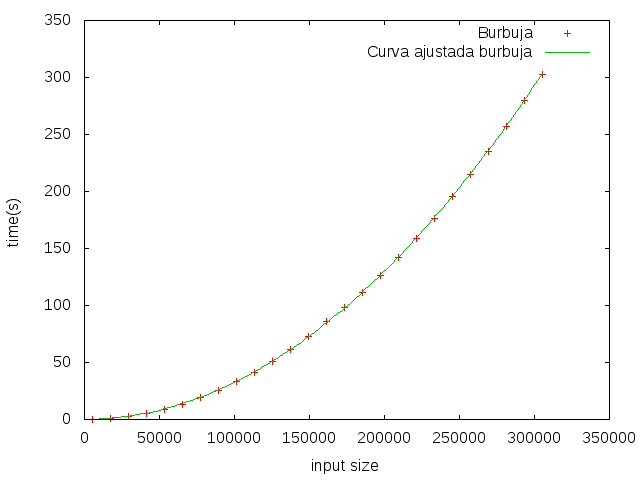
\includegraphics[width=1\textwidth]{burbuja_ajustado.png}
					\caption{Gráfica del algoritmo \textit{Burbuja} y su función ajustada. Compilación sin optimización. Intel® Core™ i7-5500U CPU @ 2.40GHz.}

				\end{figure}

\newpage

			\subsubsection{Algoritmo de Inserción.}

				\par
				Aquí podemos ver el crecimiento que presenta el algoritmo de Inserción conforme aumenta el volumen de la entrada:

				\begin{figure}[h]

					\centering
					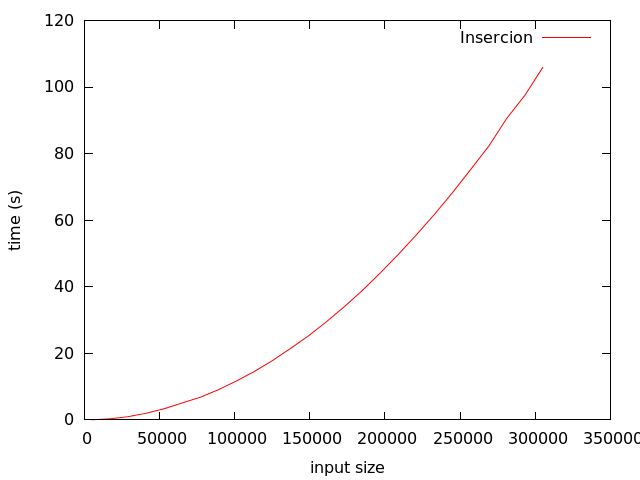
\includegraphics[width=1\textwidth]{insercion.png}
					\caption{Gráfica del algoritmo de Inserción. Compilación sin optimización. Intel® Core™ i7-5500U CPU @ 2.40GHz.}

				\end{figure}

				\par
				Mediante el análisis híbrido obtenemos las siguientes constantes ocultas:

				\begin{itemize}

					\item
					$a$ $=$ $1.14055\cdot 10^{-9}$
					\item
					$b$ $=$ $-6.62085\cdot 10^{-7}$
					\item
					$c$ $=$ $0.0683299$

				\end{itemize}

				\par
				$f(x)$ $=$ $ 1.14055\cdot 10^{-9}\cdot x^2 - 6.62085\cdot 10^{-7}\cdot x+ 0.0683299$

\newpage

				\par
				La gráfica de los tiempos obtenidos junto con la función ajustada es la siguiente:

				\begin{figure}[h]

					\centering
					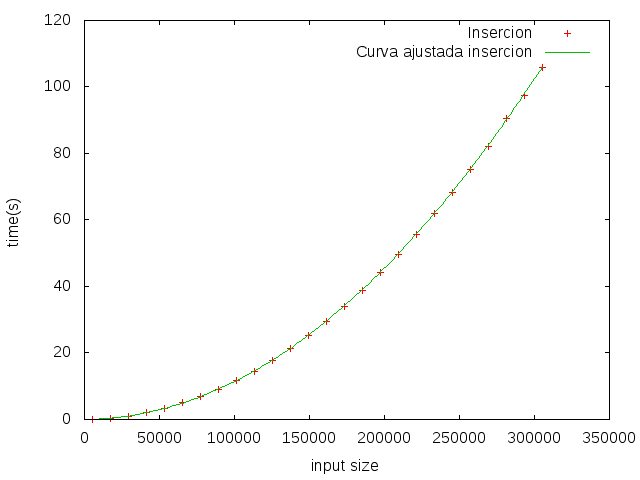
\includegraphics[width=1\textwidth]{insercion_ajustado.png}
					\caption{Gráfica del algoritmo de Inserción y su función ajustada. Compilación sin optimización. Intel® Core™ i7-5500U CPU @ 2.40GHz.}

				\end{figure}

\newpage

			\subsubsection{Algoritmo de Selección.}

				\par
				La curva que presenta el algoritmo de Selección conforme incrementamos el tamaño de los datos es la siguiente:

				\begin{figure}[h]

					\centering
					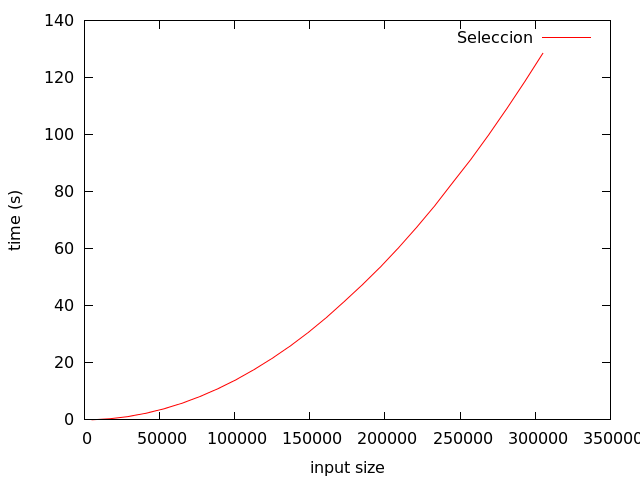
\includegraphics[width=1\textwidth]{seleccion.png}
					\caption{Gráfica del algoritmo de Selección. Compilación sin optimización. Intel® Core™ i7-5500U CPU @ 2.40GHz.}

				\end{figure}

				\par
				Las constantes ocultas que aproximan $f(x)$ a los datos representados en la gráfica anterior son:

				\begin{itemize}

					\item
					$a$ $=$ $1.3791\cdot 10^{-9}$
					\item
					$b$ $=$ $8.02857\cdot 10^{-7}$
					\item
					$c$ $=$ $-0.0274645$

				\end{itemize}

				\par
				$f(x)$ $=$ $ 1.3791\cdot 10^{-9}\cdot x^2 + 8.02857\cdot 10^{-7}\cdot x - 0.0274645$

\newpage

				\par
				Aquí podemos ver el ajuste de los datos a la función calculada en el apartado anterior:

				\begin{figure}[h]

					\centering
					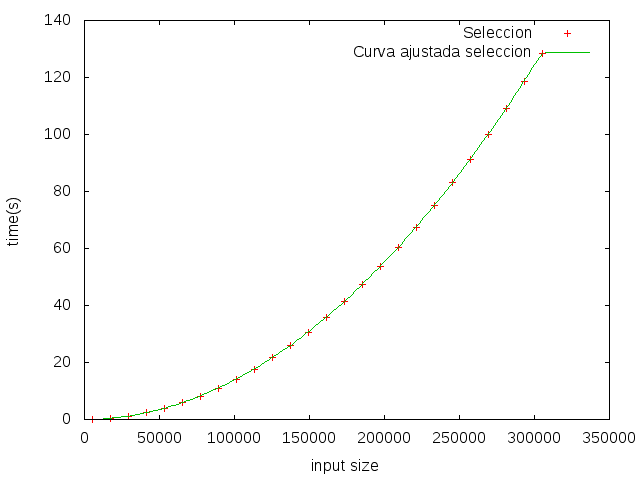
\includegraphics[width=1\textwidth]{seleccion_ajustado.png}
					\caption{Gráfica del algoritmo de Selección y su función ajustada. Compilación sin optimización. Intel® Core™ i7-5500U CPU @ 2.40GHz.}

				\end{figure}

\newpage

			\subsubsection{Comparativa de los algoritmos de O($n^2$).}

				\par
				En primer lugar, presentamos una gráfica para observar mejor las diferencias de rendimiento entre los distintos algoritmos:

				\begin{figure}[h]

					\centering
					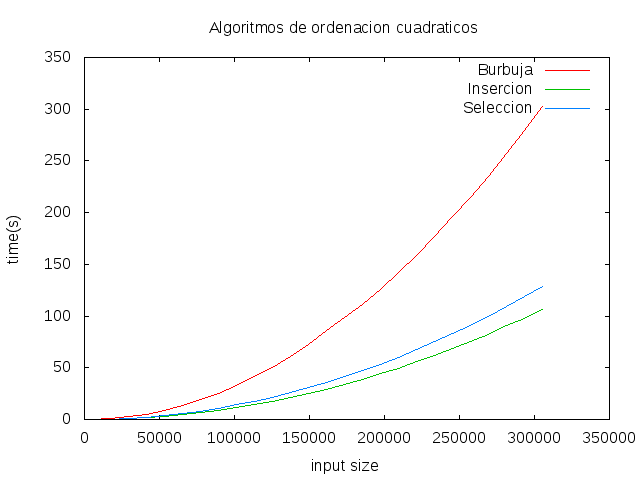
\includegraphics[width=1\textwidth]{Ncuadrado.png}
					\caption{Gráfica comparativa de los algoritmos de ordenación cuadráticos. Compilación sin optimización. Intel® Core™ i7-5500U CPU @ 2.40GHz.}

				\end{figure}

				\par
				Aunque los tres algoritmos tienen una eficiencia de O($n^2$) y, según la notación asintótica, los tres algoritmos tardarían potencialmente lo mismo, en esta gráfica podemos ver que no es así. El algoritmo \textit{Burbuja} se diferencia rápidamente de los otros y presenta un crecimiento mucho más rápido, algo que veíamos ya con las constantes ocultas anteriores; por lo tanto, es bastante más costoso aun teniendo el mismo orden de eficiencia. También podemos comprobar que, si bien Inserción y Selección al principio tienen una eficiencia muy parecida, conforme se aumenta el volumen de datos el de Selección resulta algo más ineficiente.

\newpage

				\par
				A continuación, la tabla de tiempos de ejecución:

				\begin{figure}[h]

					\centering

					\begin{tabular}{| >{\centering\arraybackslash}m{1in} | >{\centering\arraybackslash}m{1in} | >{\centering\arraybackslash}m{1in} | >{\centering\arraybackslash}m{1in} |}

						\hline
						\textbf{Tamaño de $n$} & \textbf{Tiempo Burbuja ($s$)} & \textbf{Tiempo Inserción ($s$)} & \textbf{Tiempo Selección ($s$)} \\
						\hline
						5000 & 0.059966 & 0.02864 & 0.035099 \\
						\hline
						17000 & 0.85589 & 0.331283 & 0.400708 \\
						\hline
						29000 & 2.5781 & 0.95447 & 1.16477 \\
						\hline
						41000 & 5.27445 & 1.98294 & 2.32755 \\
						\hline
						53000 & 8.96341 & 3.33574 & 3.88535 \\
						\hline
						65000 & 13.5704 & 5.05818 & 5.84135 \\
						\hline
						77000 & 19.1414 & 6.77307 & 8.19565 \\
						\hline
						89000 & 25.6015 & 9.02627 & 10.9497 \\
						\hline
						101000 & 33.0638 & 11.6468 & 14.0946 \\
						\hline
						113000 & 41.4656 & 14.5133 & 17.6426 \\
						\hline
						125000 & 50.6853 & 17.7904 & 21.5895 \\
						\hline
						137000 & 61.1032 & 21.4265 & 25.9274 \\
						\hline
						149000 & 72.5801 & 25.2194 & 30.6664 \\
						\hline
						161000 & 85.8144 & 29.4826 & 35.8634 \\
						\hline
						173000 & 98.377 & 34.036 & 41.5437 \\
						\hline
						185000 & 111.575 & 38.9165 & 47.4152 \\
						\hline
						197000 & 126.05 & 44.2132 & 53.6117 \\
						\hline
						209000 & 141.952 & 49.7696 & 60.3333 \\
						\hline
						221000 & 158.771 & 55.6643 & 67.4613 \\
						\hline
						233000 & 176.711 & 61.8095 & 74.9793 \\
						\hline
						245000 & 195.801 & 68.3384 & 83.151 \\
						\hline
						257000 & 214.78 & 75.2418 & 91.2287 \\
						\hline
						269000 & 235.283 & 82.2099 & 99.932 \\
						\hline
						281000 & 257.423 & 90.579 & 109.087 \\
						\hline
						293000 & 279.65 & 97.4804 & 118.599 \\
						\hline
						305000 & 302.741 & 105.925 & 128.49 \\
						\hline

					\end{tabular}

				\end{figure}

\newpage

		\subsection{Algoritmos de orden O($n\log_{}n$).}

			\par
			En esta sección, analizaremos la eficiencia empírica e híbrida de los algoritmos \textit{Heapsort}, \textit{Mergesort} y \textit{Quicksort}.

			\par
			En los cálculos de eficiencia híbrida ajustaremos la función: $ax \log_{}(x)$.

			\subsubsection{Algoritmo \textit{Heapsort}.}

				\par
				Éste es el crecimiento que se experimenta cuando el algoritmo \textit{Heapsort} maneja diferentes tamaños de datos:

				\begin{figure}[h]

					\centering
					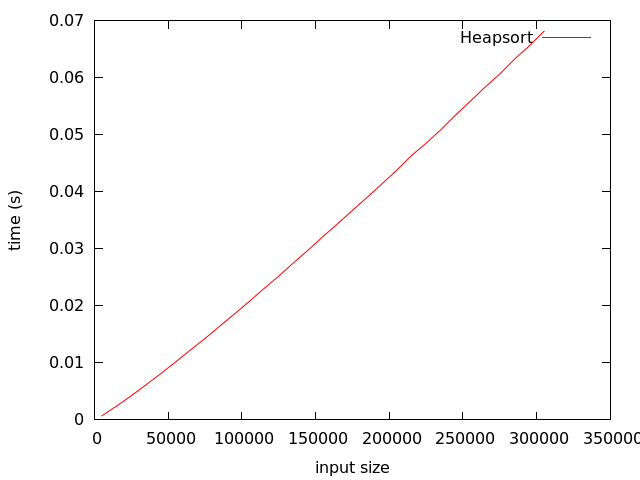
\includegraphics[width=1\textwidth]{heapsort.png}
					\caption{Gráfica del algoritmo \textit{Heapsort}. Compilación sin optimización. Intel® Core™ i7-5500U CPU @ 2.40GHz.}

				\end{figure}

				\par
				Para ajustar $f(x)$ a la gráfica anterior, necesitamos los siguientes valores:

				\begin{itemize}

					\item
					$a$ $=$ $1.7522\cdot 10^{-8}$

				\end{itemize}

				\par
				$f(x)$ $=$ $ 1.7522\cdot 10^{-8}\cdot x \cdot \log_{}(x)$

\newpage

				\par
				Si representamos los datos junto con la función ajustada, obtenemos la siguiente gráfica:

				\begin{figure}[h]

					\centering
					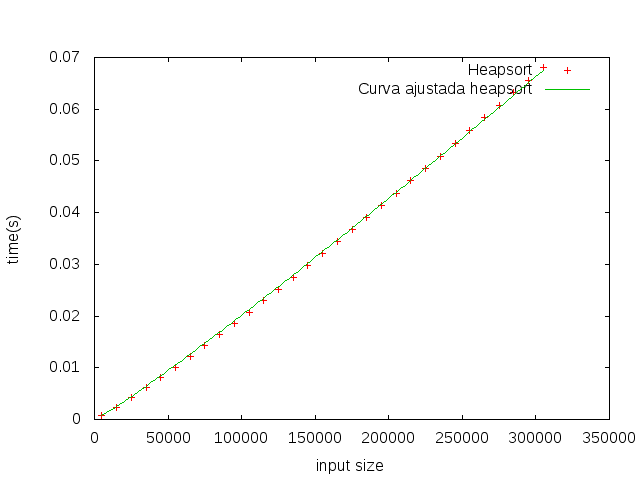
\includegraphics[width=1\textwidth]{heapsort_ajustado.png}
					\caption{Gráfica del algoritmo \textit{Heapsort} y su función ajustada. Compilación sin optimización. Intel® Core™ i7-5500U CPU @ 2.40GHz.}

				\end{figure}

\newpage

			\subsubsection{Algoritmo \textit{Mergesort}.}

				\par
				A continuación mostramos gráficamente los tiempos de ejecución del algoritmo \textit{Mergesort}:

				\begin{figure}[h]

					\centering
					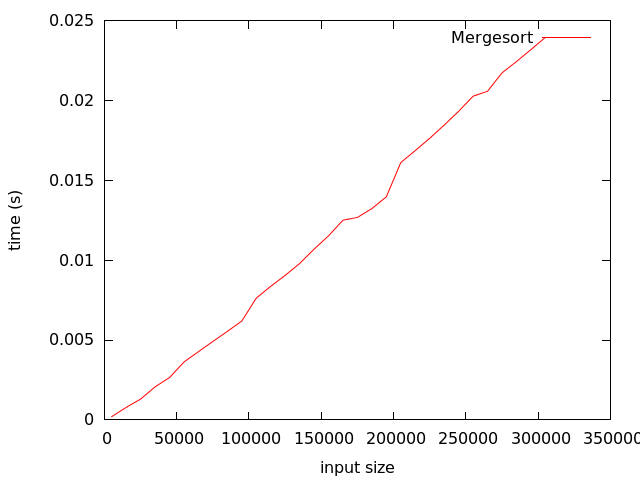
\includegraphics[width=1\textwidth]{mergesort.png}
					\caption{Gráfica del algoritmo \textit{Mergesort}. Compilación sin optimización. Intel® Core™ i7-5500U CPU @ 2.40GHz.}

				\end{figure}

				\par
				El resultado que da el análisis híbrido del algoritmo \textit{Mergesort} es:

				\begin{itemize}

					\item
					$a$ $=$ $6.23896\cdot 10^{-9}$

				\end{itemize}

				\par
				$f(x)$ $=$ $ 6.23896\cdot 10^{-9}\cdot x \cdot \log_{}(x)$

\newpage

				\par
				Al representar la curva de $f(x)$ ajustada y los datos empíricos, obtenemos:

				\begin{figure}[h]

					\centering
					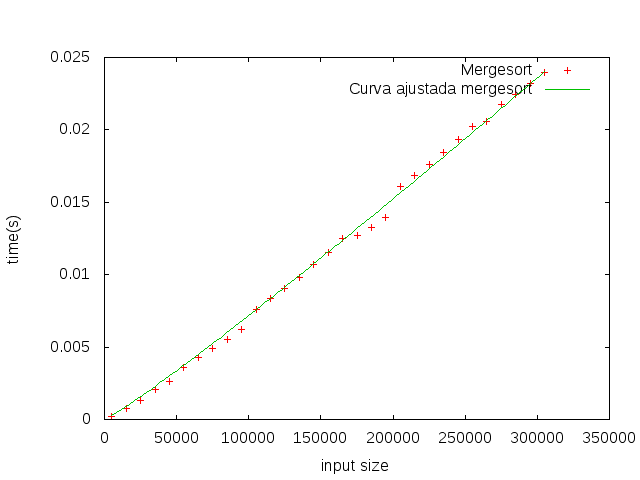
\includegraphics[width=1\textwidth]{mergesort_ajustado.png}
					\caption{Gráfica del algoritmo \textit{Mergesort} y su función ajustada. Compilación sin optimización. Intel® Core™ i7-5500U CPU @ 2.40GHz.}

				\end{figure}

\newpage

			\subsubsection{Algoritmo \textit{Quicksort}.}

				\par
				En la siguiente gráfica podemos observar el crecimiento que presenta el algoritmo \textit{Quicksort}:

				\begin{figure}[h]

					\centering
					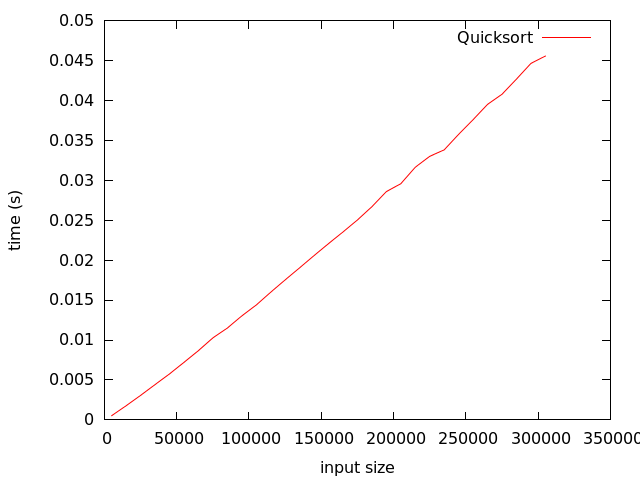
\includegraphics[width=1\textwidth]{quicksort.png}
					\caption{Gráfica del algoritmo \textit{Quicksort}. Compilación sin optimización. Intel® Core™ i7-5500U CPU @ 2.40GHz.}

				\end{figure}

				\par
				El análisis híbrido de los datos representados en la gráfica produce el siguiente resultado:

				\begin{itemize}

					\item
					$a$ $=$ $1.18815\cdot 10^{-8}$

				\end{itemize}

				\par
				$f(x)$ $=$ $ 1.18815\cdot 10^{-8}\cdot x \cdot \log_{}(x)$

\newpage

				\par
				En la siguiente gráfica podemos ver el ajuste de $f(x)$ a las sucesivas ejecuciones del algoritmo:

				\begin{figure}[h]

					\centering
					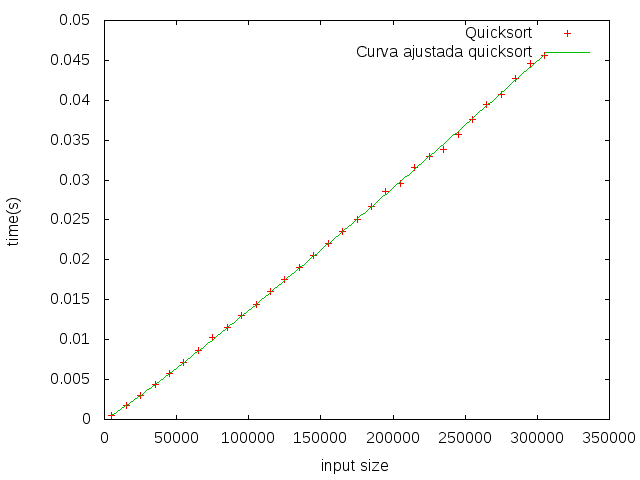
\includegraphics[width=1\textwidth]{quicksort_ajustado.png}
					\caption{Gráfica del algoritmo \textit{Quicksort} y su función ajustada. Compilación sin optimización. Intel® Core™ i7-5500U CPU @ 2.40GHz.}

				\end{figure}

\newpage

			\subsubsection{Comparativa de los algoritmos de O($n\log_{}n$)}

				\par
				En primer lugar, presentamos una gráfica para observar mejor las diferencias de rendimiento entre los distintos algoritmos:

				\begin{figure}[h]

					\centering
					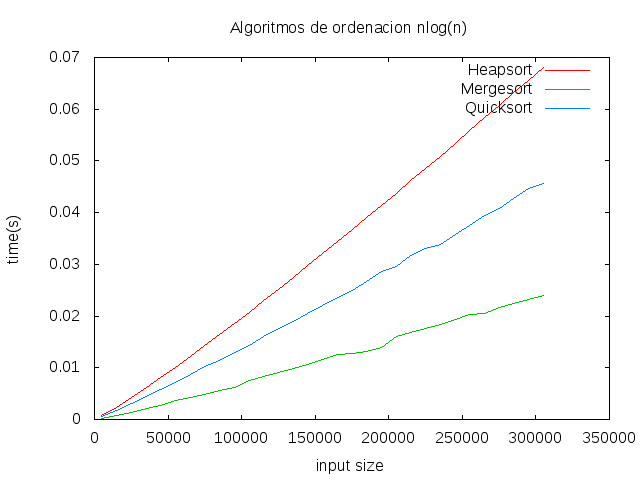
\includegraphics[width=1\textwidth]{Nlogn.png}
					\caption{Gráfica comparativa de los algoritmos de ordenación cuadráticos. Compilación sin optimización. Intel® Core™ i7-5500U CPU @ 2.40GHz.}

				\end{figure}

				\par
				Los datos muestran que, en principio, el algoritmo \textit{Mergesort} es el mejor, seguido de \textit{Quicksort} y \textit{Heapsort}. Sin embargo, los tamaños están ajustados con el objetivo de poder compararlos con los de los algoritmos de ordenación cuadráticos, por lo que son muy pequeños para un orden O($n\log_{}n$) y podrían no ser representativos de la eficiencia en condiciones más realistas.

\newpage

				\par
				A continuación, la tabla de tiempos de ejecución:

				\begin{figure}[h]

					\centering

					\begin{tabular}{| >{\centering\arraybackslash}m{1in} | >{\centering\arraybackslash}m{1in} | >{\centering\arraybackslash}m{1in} | >{\centering\arraybackslash}m{1in} |}

						\hline
						\textbf{Tamaño de $n$} & \textbf{Tiempo \textit{Heapsort} ($s$)} & \textbf{Tiempo \textit{Mergesort} ($s$)} & \textbf{Tiempo \textit{Quicksort} ($s$)} \\
						\hline
						15000 & 0.002412 & 0.000780945 & 0.001771 \\
						\hline
						25000 & 0.004227 & 0.00129756 & 0.003062 \\
						\hline
						35000 & 0.006153 & 0.00206483 & 0.004411 \\
						\hline
						45000 & 0.008111 & 0.00264398 & 0.005754 \\
						\hline
						55000 & 0.01014 & 0.00361779 & 0.007196 \\
						\hline
						65000 & 0.012223 & 0.00426566 & 0.008663 \\
						\hline
						75000 & 0.014257 & 0.00490762 & 0.010267 \\
						\hline
						85000 & 0.016429 & 0.00553744 & 0.011495 \\
						\hline
						95000 & 0.018575 & 0.00618519 & 0.013014 \\
						\hline
						105000 & 0.020746 & 0.00762148 & 0.014378 \\
						\hline
						115000 & 0.023012 & 0.00836004 & 0.015983 \\
						\hline
						125000 & 0.025217 & 0.00904335 & 0.017521 \\
						\hline
						135000 & 0.027526 & 0.0097835 & 0.01904 \\
						\hline
						145000 & 0.029776 & 0.0106871 & 0.020568 \\
						\hline
						155000 & 0.032133 & 0.0115184 & 0.022066 \\
						\hline
						165000 & 0.034391 & 0.0125027 & 0.023528 \\
						\hline
						175000 & 0.036719 & 0.0126728 & 0.02503 \\
						\hline
						185000 & 0.039012 & 0.0132283 & 0.026689 \\
						\hline
						195000 & 0.04136 & 0.0139646 & 0.028577 \\
						\hline
						205000 & 0.043756 & 0.0161064 & 0.029569 \\
						\hline
						215000 & 0.046311 & 0.0168623 & 0.031633 \\
						\hline
						225000 & 0.048505 & 0.0176279 & 0.032997 \\
						\hline
						235000 & 0.050869 & 0.018451 & 0.033803 \\
						\hline
						245000 & 0.053452 & 0.0193148 & 0.035749 \\
						\hline
						255000 & 0.055863 & 0.0202648 & 0.037587 \\
						\hline
						265000 & 0.058341 & 0.0205711 & 0.039503 \\
						\hline
						275000 & 0.060633 & 0.0217225 & 0.040769 \\
						\hline
						285000 & 0.063236 & 0.0224305 & 0.042672 \\
						\hline
						295000 & 0.065567 & 0.0231778 & 0.044629 \\
						\hline
						305000 & 0.068137 & 0.0239459 & 0.04555 \\
						\hline

					\end{tabular}

				\end{figure}

\newpage

		\subsection{Comparativa general de algoritmos de ordenación.}

			\par
			A continuación, una gráfica que contrasta los tiempos de los seis algoritmos analizados previamente:

			\begin{figure}[h]

				\centering
				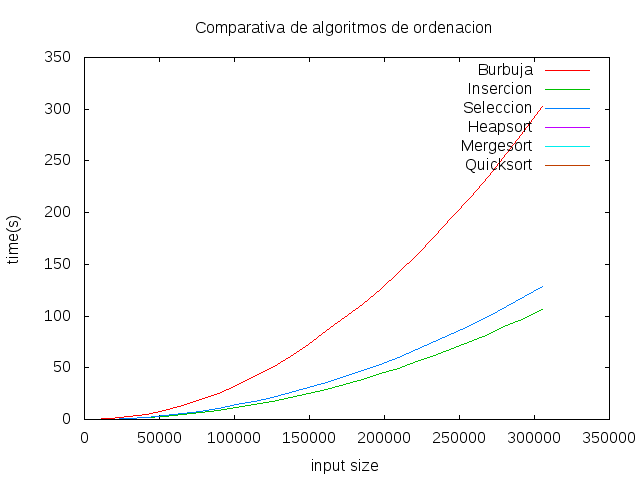
\includegraphics[width=1\textwidth]{Comparativa.png}
				\caption{Gráfica comparativa de los algoritmos de ordenación. Compilación sin optimización. Intel® Core™ i7-5500U CPU @ 2.40GHz.}

			\end{figure}

			En esta gráfica se puede ver la gran diferencia que hay entre una eficiencia de $n^2$ y una de $n\log_{}n$, tanta que ni siquiera se aprecian en la gráfica las curvas de los algoritmos \textit{Heapsort}, \textit{Mergesort} y \textit{Quicksort}. Mientras que para tamaños de varios cientos de miles los algoritmos de O($n^2$) tardan varios minutos, los de O($n\log_{}n$) terminan en cuestión de centésimas de segundo. Esta diferencia es una clara demostración de la importancia de elegir un algoritmo con el menor orden posible (aunque teniendo cuidado con las constantes ocultas), ya que no es sólo cuestión de unos pocos segundos.

\newpage

	\section{Algoritmo de Floyd.}

		\subsection{Descripción breve.}

			\par
			El algoritmo de Floyd se utiliza para encontrar el camino más corto entre cada par de nodos en un grafo dirigido. Su orden es O($n^3$).

		\subsection{Tabla de tiempos de ejecución.}

			\par
			Los resultados para $n$ en el rango [100,1550] son:

			\vspace{0.5cm}

			\begin{figure}[h]

				\centering

				\begin{tabular}{| >{\centering\arraybackslash}m{1in} | >{\centering\arraybackslash}m{1in} |}

					\hline
					\textbf{Tamaño de $n$} & \textbf{Tiempo ($s$)} \\
					\hline
					100 & 0.006108 \\
					\hline
					150 & 0.020072 \\
					\hline
					200 & 0.047014 \\
					\hline
					250 & 0.091181 \\
					\hline
					300 & 0.156999 \\
					\hline
					350 & 0.248901 \\
					\hline
					400 & 0.370784 \\
					\hline
					450 & 0.528139 \\
					\hline
					500 & 0.722818 \\
					\hline
					550 & 0.961853 \\
					\hline
					600 & 1.24689 \\
					\hline
					650 & 1.58944 \\
					\hline
					700 & 1.99242 \\
					\hline
					750 & 2.431558 \\
					\hline
					800 & 2.96925 \\
					\hline
					850 & 3.68909 \\
					\hline
					900 & 4.24717 \\
					\hline
					950 & 5.02479 \\
					\hline
					1000 & 5.88652 \\
					\hline
					1050 & 6.81454 \\
					\hline
					1100 & 7.88513 \\
					\hline
					1150 & 9.0024 \\
					\hline
					1200 & 10.247 \\
					\hline
					1250 & 11.5879 \\
					\hline
					1300 & 12.99 \\
					\hline
					1350 & 14.5377 \\
					\hline
					1400 & 16.2152 \\
					\hline
					1450 & 18.0179 \\
					\hline
					1500 & 19.9648 \\
					\hline
					1550 & 21.9085 \\
					\hline

				\end{tabular}

			\end{figure}

		\subsection{Gráfica del algoritmo.}

			\par
			Los tiempos de ejecución representados en forma de curva son:

			\begin{figure}[h]

				\centering
				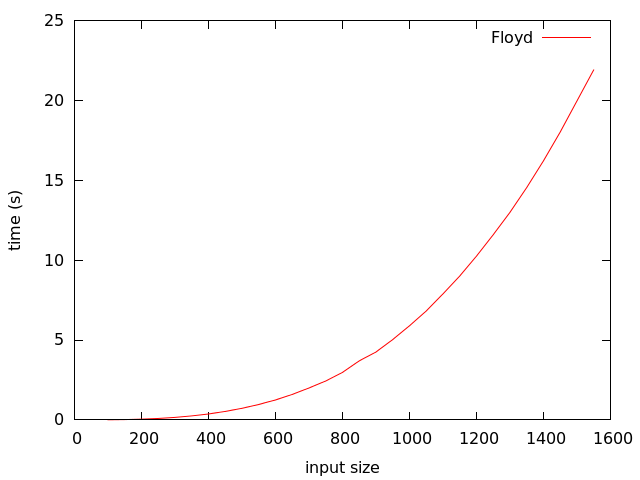
\includegraphics[width=1\textwidth]{floyd.png}
				\caption{Gráfica del algoritmo de Floyd. Compilación sin optimización. Intel® Core™ i7-5500U CPU @ 2.40GHz.}

			\end{figure}

		\subsection{Análisis híbrido.}

			\par
			Procedemos a ajustar los datos obtenidos a la siguiente función: $ax^3+bx^2+cx+d$.

			\begin{itemize}

					\item
					$a$ $=$ $5.69357\cdot 10^{-9}$
					\item
					$b$ $=$ $5.61065\cdot 10^{-7}$
					\item
					$c$ $=$ $-0.000409355$
					\item
					$d$ $=$ $0.0612349$

			\end{itemize}

			\par
			$f(x)$ $=$ $ 5.69357\cdot 10^{-9}\cdot x^3 + 5.61065\cdot 10^{-7}\cdot x^2 - 0.000409355\cdot x+ 0.0612349$

\newpage

			\par
			La representación gráfica del análisis híbrido es la siguiente:

			\begin{figure}[h]

				\centering
				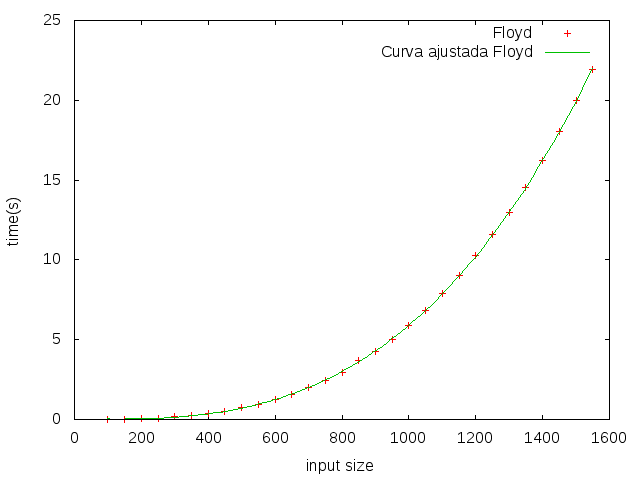
\includegraphics[width=1\textwidth]{floyd_ajustado.png}
				\caption{Gráfica del algoritmo de Floyd y su función ajustada. Compilación sin optimización. Intel® Core™ i7-5500U CPU @ 2.40GHz.}

			\end{figure}

\newpage

	\section{Algoritmo de las torres de Hanoi.}

		\subsection{Descripción breve.}

			\par
			El problema de las torres de Hanoi consiste en mover una serie de discos de radio creciente desde una estaca a otra de un tablero con ayuda de una tercera. Los movimientos se deben hacer teniendo en cuenta que ningún disco puede estar encima de otro de menor tamaño, que sólo se puede mover uno a la vez y que sólo se puede mover el que esté encima de los demás en su correspondiente estaca. El orden de este algoritmo es O($2^n$).

		\subsection{Tabla de tiempos de ejecución.}

			\par
			A continuación se muestran los resultados para $n$ en el rango [8,33]:

			\vspace{0.5cm}

			\begin{figure}[h]

				\centering

				\begin{tabular}{| >{\centering\arraybackslash}m{1in} | >{\centering\arraybackslash}m{1in} |}

					\hline
					\textbf{Tamaño de $n$} & \textbf{Tiempo ($s$)} \\
					\hline
					8 & 0.000002 \\
					\hline
					9 & 0.000004 \\
					\hline
					10 & 0.000007 \\
					\hline
					11 & 0.000014 \\
					\hline
					12 & 0.000027 \\
					\hline
					13 & 0.000053 \\
					\hline
					14 & 0.000105 \\
					\hline
					15 & 0.000223 \\
					\hline
					16 & 0.000435 \\
					\hline
					17 & 0.001049 \\
					\hline
					18 & 0.001676 \\
					\hline
					19 & 0.00336 \\
					\hline
					20 & 0.006766 \\
					\hline
					21 & 0.013481 \\
					\hline
					22 & 0.026936 \\
					\hline
					23 & 0.053744 \\
					\hline
					24 & 0.107664 \\
					\hline
					25 & 0.215053 \\
					\hline
					26 & 0.429739 \\
					\hline
					27 & 0.859611 \\
					\hline
					28 & 1.71886 \\
					\hline
					29 & 3.43784 \\
					\hline
					30 & 6.88029 \\
					\hline
					31 & 13.7576 \\
					\hline
					32 & 27.6634 \\
					\hline
					33 & 55.0232 \\
					\hline

				\end{tabular}

			\end{figure}

		\subsection{Gráfica del algoritmo.}

			\par
			La siguiente curva corresponde a la ejecución sucesiva del algoritmo de las torres de Hanoi:

			\begin{figure}[h]

				\centering
				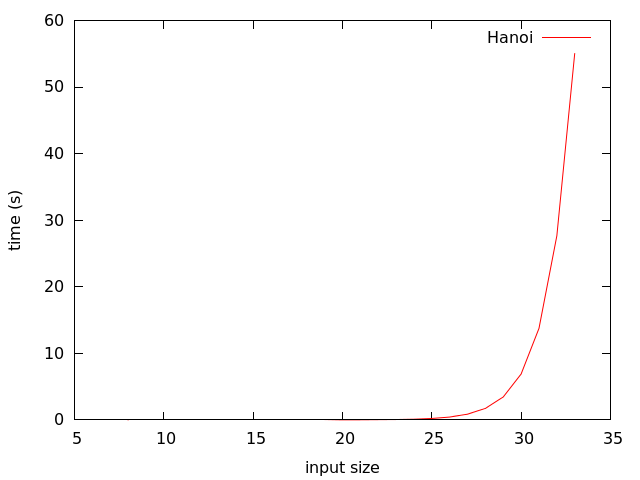
\includegraphics[width=1\textwidth]{hanoi.png}
				\caption{Gráfica del algoritmo de las torres de Hanoi. Compilación sin optimización. Intel® Core™ i7-5500U CPU @ 2.40GHz.}

			\end{figure}

			\par
			Este algoritmo, al ser de orden O($2^n$), resulta tremendamente ineficiente. En la gráfica vemos que para valores muy pequeños ni se aprecia el tiempo que tarda, pero a partir de tan sólo un tamaño de 25, la curva empieza a experimentar un crecimiento
			enorme. Con un tamaño de únicamente 40 (que es un valor muy pequeño en los otros algoritmos), el algoritmo de Hanoi tardaría unas 2 horas; para un tamaño de 50 tendríamos que esperar unos 3 meses para ver a nuestro algoritmo terminar.

\newpage

		\subsection{Análisis híbrido.}

			\par
			En esta sección vamos a ajustar los datos obtenidos a la siguiente función: $a\cdot b^x$.

			\begin{itemize}

					\item
					$a$ $=$ $6.76475\cdot 10^{-9}$
					\item
					$b$ $=$ $1.99673$

			\end{itemize}

			\par
			$f(x)$ $=$ $ 6.76475\cdot 10^{-9}\cdot 1.99673^x$

			\vspace{5mm}

			\par
			Al representar los tiempos de ejecución y la función ajustada a ellos, obtenemos:

			\begin{figure}[h]

				\centering
				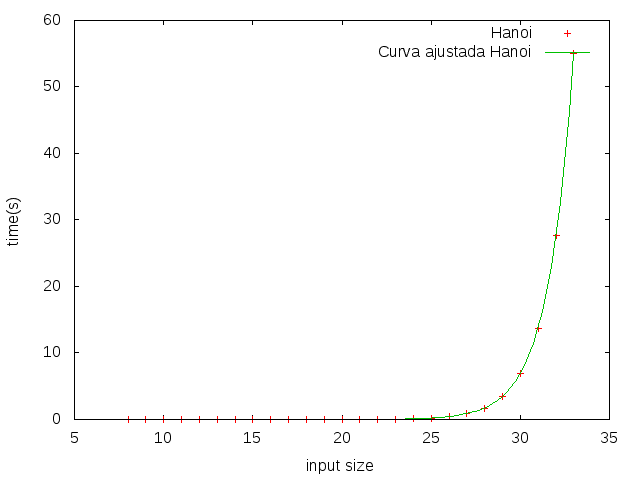
\includegraphics[width=1\textwidth]{hanoi_ajustado.png}
				\caption{Gráfica del algoritmo de las torres de Hanoi y su función ajustada. Compilación sin optimización. Intel® Core™ i7-5500U CPU @ 2.40GHz.}

			\end{figure}

\newpage

	\section{Análisis de parámetros externos.}

		\subsection{Nivel de optimización al compilar.}

			\par
			En esta sección estudiaremos el efecto que tienen distintas optimizaciones al compilar en los diferentes tipos de algoritmos.

			\subsubsection{Algoritmos de orden O($n^2$).}

				\par
				Para realizar este análisis, tomaremos el algoritmo de Selección como representante de los algoritmos cuadráticos.

				\par
				En la siguiente gráfica podemos observar las diferencias en el tiempo de ejecución, que son bastante notables en los casos de optimización de nivel 1 y 2; por su parte, el nivel 3 no sólo no aporta ninguna mejora sino que pierde casi la mitad de efectividad.

				\begin{figure}[h]

					\centering
					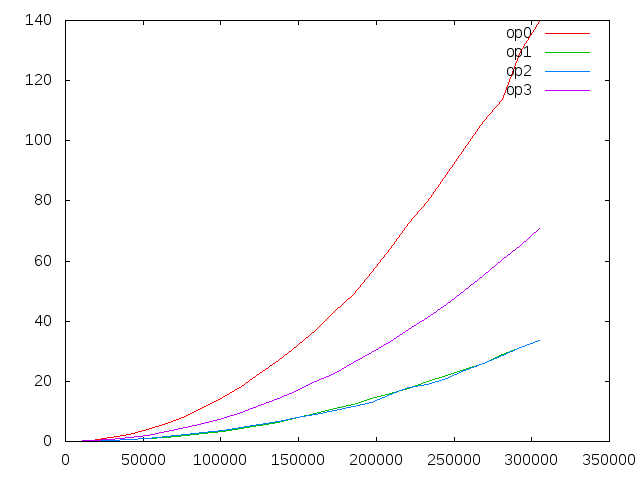
\includegraphics[width=1\textwidth]{seleccion_opt.png}
					\caption{Gráfica del algoritmo de Selección con distintas opciones de compilación. Intel® Core™ i5-2320 CPU @ 3.00GHz.}

				\end{figure}

\newpage

				\par
				Para mayor claridad, adjuntamos la tabla de tiempos:

				\begin{figure}[h]

					\centering

					\begin{tabular}{| >{\centering\arraybackslash}m{1in} | >{\centering\arraybackslash}m{1in} | >{\centering\arraybackslash}m{1in} | >{\centering\arraybackslash}m{1in} | >{\centering\arraybackslash}m{1in} |}

						\hline
						\textbf{Tamaño de $n$} & \textbf{Nivel 0} & \textbf{Nivel 1} & \textbf{Nivel 2} & \textbf{Nivel 3} \\
						\hline
						5000 & 0.036124 & 0.009041 & 0.00938 & 0.019137 \\
						\hline
						17000 & 0.414943 & 0.09991 & 0.11193 & 0.21985 \\
						\hline
						29000 & 1.20676 & 0.287832 & 0.312588 & 0.64235 \\
						\hline
						41000 & 2.40054 & 0.569582 & 0.620342 & 1.28279 \\
						\hline
						53000 & 4.01078 & 0.948723 & 1.04029 & 2.14851 \\
						\hline
						65000 & 6.03459 & 1.43653 & 1.5454 & 3.20979 \\
						\hline
						77000 & 8.46338 & 2.02502 & 2.19426 & 4.50478 \\
						\hline
						89000 & 11.3048 & 2.68759 & 2.84887 & 6.02035 \\
						\hline
						101000 & 14.5591 & 3.47514 & 3.65536 & 7.7515 \\
						\hline
						113000 & 18.2305 & 4.32426 & 4.66081 & 9.8025 \\
						\hline
						125000 & 22.5115 & 5.25863 & 5.53469 & 11.9881 \\
						\hline
						137000 & 27.0404 & 6.35793 & 6.71818 & 14.3984 \\
						\hline
						149000 & 31.9853 & 7.85416 & 7.97568 & 17.0428 \\
						\hline
						161000 & 37.0007 & 9.25359 & 9.12481 & 19.8977 \\
						\hline
						173000 & 43.0687 & 10.927 & 10.3218 & 22.7449 \\
						\hline
						185000 & 48.9193 & 12.2514 & 11.5484 & 26.1665 \\
						\hline
						197000 & 56.0373 & 14.3025 & 13.0519 & 29.4895 \\
						\hline
						209000 & 64.295 & 16.0266 & 15.6726 & 33.365 \\
						\hline
						221000 & 72.4991 & 17.7103 & 17.9539 & 37.1059 \\
						\hline
						233000 & 79.7657 & 19.8308 & 18.9754 & 41.2455 \\
						\hline
						245000 & 88.8895 & 21.9423 & 20.8413 & 45.6001 \\
						\hline
						257000 & 97.5091 & 24.0771 & 23.7747 & 50.1777 \\
						\hline
						269000 & 106.297 & 25.9644 & 25.8485 & 55.3627 \\
						\hline
						281000 & 113.799 & 28.8626 & 28.6332 & 60.4656 \\
						\hline
						293000 & 129.573 & 31.3742 & 31.4038 & 65.2064 \\
						\hline
						305000 & 139.702 & 33.5263 & 33.49 & 70.7969 \\
						\hline

					\end{tabular}

				\end{figure}

\newpage

			\subsubsection{Algoritmos de orden O($n\log_{}n$).}

				\par
				En este caso, el algoritmo \textit{Quicksort} servirá como caso de estudio para los algoritmos de orden O($n\log_{}n$).

				\par
				Mediante la gráfica podemos comprobar que la optimización a distintos niveles puede ser beneficiosa pero no hay una gran diferencia de rendimiento. En particular, la optimización de nivel 1 parece ser peor que la de nivel 0 según los datos obtenidos.

				\begin{figure}[h]

					\centering
					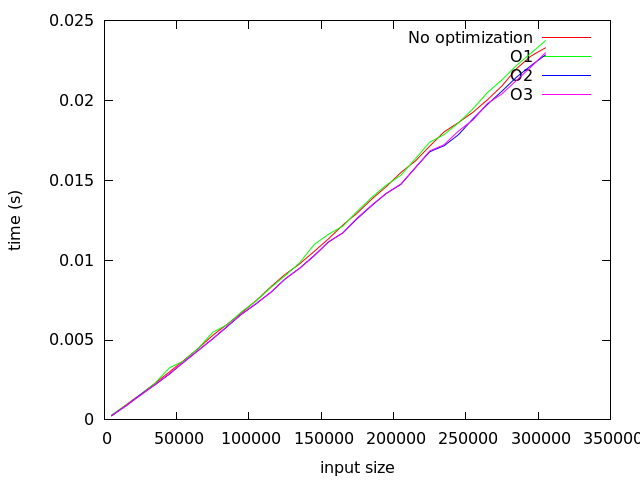
\includegraphics[width=1\textwidth]{quicksort_opt.png}
					\caption{Gráfica del algoritmo \textit{Quicksort} con distintas opciones de compilación. Intel® Core™ i7-5500U CPU @ 2.40GHz.}

				\end{figure}

\newpage

				\par
				Para mayor claridad, adjuntamos la tabla de tiempos:

				\begin{figure}[h]

					\centering

					\begin{tabular}{| >{\centering\arraybackslash}m{1in} | >{\centering\arraybackslash}m{1in} | >{\centering\arraybackslash}m{1in} | >{\centering\arraybackslash}m{1in} | >{\centering\arraybackslash}m{1in} |}

						\hline
						\textbf{Tamaño de $n$} & \textbf{Nivel 0} & \textbf{Nivel 1} & \textbf{Nivel 2} & \textbf{Nivel 3} \\
						\hline
						15000 & 0.001771 & 0.000928 & 0.000882 & 0.000882 \\
						\hline
						25000 & 0.003062 & 0.001575 & 0.001576 & 0.001547 \\
						\hline
						35000 & 0.004411 & 0.002297 & 0.002194 & 0.002204 \\
						\hline
						45000 & 0.005754 & 0.003259 & 0.002868 & 0.0029 \\
						\hline
						55000 & 0.007196 & 0.003694 & 0.003621 & 0.003622 \\
						\hline
						65000 & 0.008663 & 0.004483 & 0.004355 & 0.004354 \\
						\hline
						75000 & 0.010267 & 0.00549 & 0.005083 & 0.005079 \\
						\hline
						85000 & 0.011495 & 0.005963 & 0.005843 & 0.005879 \\
						\hline
						95000 & 0.013014 & 0.006773 & 0.006628 & 0.00663 \\
						\hline
						105000 & 0.014378 & 0.00745 & 0.007269 & 0.007295 \\
						\hline
						115000 & 0.015983 & 0.008277 & 0.007978 & 0.007971 \\
						\hline
						125000 & 0.017521 & 0.009028 & 0.00882 & 0.008821 \\
						\hline
						135000 & 0.01904 & 0.009832 & 0.009495 & 0.00948 \\
						\hline
						145000 & 0.020568 & 0.010966 & 0.010287 & 0.010253 \\
						\hline
						155000 & 0.022066 & 0.011623 & 0.011137 & 0.011144 \\
						\hline
						165000 & 0.023528 & 0.012134 & 0.011709 & 0.011721 \\
						\hline
						175000 & 0.02503 & 0.01307 & 0.012608 & 0.01265 \\
						\hline
						185000 & 0.026689 & 0.013931 & 0.013422 & 0.013448 \\
						\hline
						195000 & 0.028577 & 0.014698 & 0.014178 & 0.01418 \\
						\hline
						205000 & 0.029569 & 0.01531 & 0.014735 & 0.014761 \\
						\hline
						215000 & 0.031633 & 0.01634 & 0.015788 & 0.01577 \\
						\hline
						225000 & 0.032997 & 0.017385 & 0.016784 & 0.016836 \\
						\hline
						235000 & 0.033803 & 0.017863 & 0.017162 & 0.017235 \\
						\hline
						245000 & 0.035749 & 0.018605 & 0.01786 & 0.01809 \\
						\hline
						255000 & 0.037587 & 0.019483 & 0.01886 & 0.018783 \\
						\hline
						265000 & 0.039503 & 0.020494 & 0.01975 & 0.019807 \\
						\hline
						275000 & 0.040769 & 0.021284 & 0.020579 & 0.020408 \\
						\hline
						285000 & 0.042672 & 0.022184 & 0.021453 & 0.021249 \\
						\hline
						295000 & 0.044629 & 0.022953 & 0.022175 & 0.022093 \\
						\hline
						305000 & 0.045557 & 0.023731 & 0.022839 & 0.022972 \\
						\hline

					\end{tabular}

				\end{figure}

\newpage

			\subsubsection{Algoritmo de Floyd.}

				\par
				Hemos hecho mediciones de tiempo con las cuatro optimizaciones para el algoritmo de Floyd, obteniendo los siguientes resultados:

				\begin{figure}[h]

					\centering
					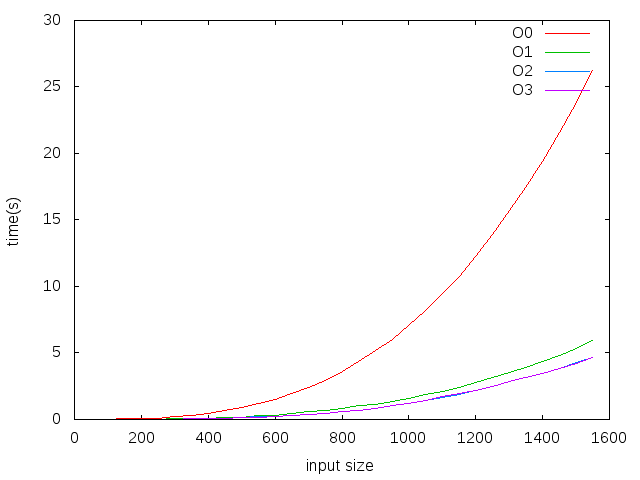
\includegraphics[width=1\textwidth]{floyd_opt.png}
					\caption{Gráfica del algoritmo de Floyd con distintas opciones de compilación. Intel® Core™ i5-4200U CPU @ 1.60GHz.}

				\end{figure}

				\par
				Podemos observar que la mejora de los niveles 1, 2 y 3 respecto al nivel 0 de optimización es más que notable, ya que reduce en más de dos tercios el tiempo de ejecución del algoritmo. Los niveles 2 y 3 de optimización apenas difieren y, aunque sí que suponen una mejora respecto al nivel 1, no es tan pronunciada.

\newpage

				\par
				Para mayor claridad, adjuntamos la tabla de tiempos:

				\begin{figure}[h]

					\centering

					\begin{tabular}{| >{\centering\arraybackslash}m{1in} | >{\centering\arraybackslash}m{1in} | >{\centering\arraybackslash}m{1in} | >{\centering\arraybackslash}m{1in} | >{\centering\arraybackslash}m{1in} |}

						\hline
						\textbf{Tamaño de $n$} & \textbf{Nivel 0} & \textbf{Nivel 1} & \textbf{Nivel 2} & \textbf{Nivel 3} \\
						\hline
						100 & 0.019403 & 0.004196 & 0.003485 & 0.004847 \\
						\hline
						150 & 0.041889 & 0.007138 & 0.009218 & 0.011776 \\
						\hline
						200 & 0.057889 & 0.012596 & 0.016861 & 0.020785 \\
						\hline
						250 & 0.111783 & 0.024436 & 0.018309 & 0.03239 \\
						\hline
						300 & 0.18856 & 0.039956 & 0.031289 & 0.034652 \\
						\hline
						350 & 0.300613 & 0.063244 & 0.052344 & 0.04781 \\
						\hline
						400 & 0.452591 & 0.093873 & 0.071509 & 0.07209 \\
						\hline
						450 & 0.676688 & 0.133829 & 0.101763 & 0.103639 \\
						\hline
						500 & 0.881619 & 0.183502 & 0.147238 & 0.138195 \\
						\hline
						550 & 1.23415 & 0.27344 & 0.189409 & 0.184614 \\
						\hline
						600 & 1.4987 & 0.314622 & 0.242244 & 0.23895 \\
						\hline
						650 & 1.93165 & 0.425116 & 0.309741 & 0.310549 \\
						\hline
						700 & 2.38591 & 0.566917 & 0.380176 & 0.38189 \\
						\hline
						750 & 2.92394 & 0.713505 & 0.473913 & 0.465974 \\
						\hline
						800 & 3.60982 & 0.792758 & 0.583663 & 0.578305 \\
						\hline
						850 & 4.3496 & 1.03309 & 0.705663 & 0.712704 \\
						\hline
						900 & 5.19879 & 1.12136 & 0.853371 & 0.859039 \\
						\hline
						950 & 6.01972 & 1.33587 & 1.0296 & 1.03618 \\
						\hline
						1000 & 7.07046 & 1.58757 & 1.22454 & 1.22418 \\
						\hline
						1050 & 8.19999 & 1.85009 & 1.43525 & 1.4529 \\
						\hline
						1100 & 9.43852 & 2.13969 & 1.67268 & 1.7051 \\
						\hline
						1150 & 10.7766 & 2.44081 & 1.91303 & 1.93099 \\
						\hline
						1200 & 12.2693 & 2.79433 & 2.18412 & 2.20683 \\
						\hline
						1250 & 13.8743 & 3.12842 & 2.50924 & 2.50058 \\
						\hline
						1300 & 15.6962 & 3.51319 & 2.82064 & 2.82453 \\
						\hline
						1350 & 17.4077 & 3.94437 & 3.16143 & 3.19427 \\
						\hline
						1400 & 19.3832 & 4.38754 & 3.4905 & 3.45987 \\
						\hline
						1450 & 21.5901 & 4.84861 & 3.85593 & 3.83144 \\
						\hline
						1500 & 23.8717 & 5.36099 & 4.28894 & 4.23618 \\
						\hline
						1550 & 26.2314 & 5.91859 & 4.6492 & 4.66486 \\
						\hline

					\end{tabular}

				\end{figure}

\newpage

			\subsubsection{Algoritmo de las torres de Hanoi.}

				\par
				Los resultados obtenidos con los diferentes niveles de optimización para el algoritmo de las torres de Hanoi pueden verse en la siguiente gráfica:

				\begin{figure}[h]

					\centering
					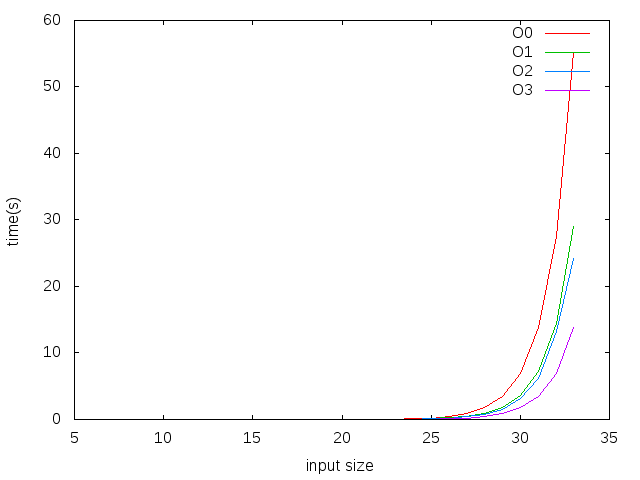
\includegraphics[width=1\textwidth]{hanoi_opt.png}
					\caption{Gráfica del algoritmo de las torres de Hanoi con distintas opciones de compilación. Intel® Core™ i7-5500U CPU @ 2.40GHz.}

				\end{figure}

				\par
				Como podemos comprobar, el nivel 1 de optimización reduce casi a la mitad el tiempo de ejecución respecto al nivel 0, lo cual es una mejora considerable si tenemos en cuenta que el algoritmo tiene un orden exponencial. El nivel 2 es ligeramente mejor que el 1, pero sin duda el que mejores tiempos obtiene es el nivel 3 de optimización, que vuelve a reducir a la mitad el tiempo respecto al nivel 1, obteniendo así casi cuatro veces mejores resultados que el nivel 0.

\newpage

				\par
				Para mayor claridad, adjuntamos la tabla de tiempos:

				\begin{figure}[h]

					\centering

					\begin{tabular}{| >{\centering\arraybackslash}m{1in} | >{\centering\arraybackslash}m{1in} | >{\centering\arraybackslash}m{1in} | >{\centering\arraybackslash}m{1in} | >{\centering\arraybackslash}m{1in} |}

						\hline
						\textbf{Tamaño de $n$} & \textbf{Nivel 0} & \textbf{Nivel 1} & \textbf{Nivel 2} & \textbf{Nivel 3} \\
						\hline
						8 & 0.00001 & 0.000002 & 0.000002 & 0.000002 \\
						\hline
						9 & 0.00001 & 0.000004 & 0.000002 & 0.000003 \\
						\hline
						10 & 0.000013 & 0.000005 & 0.000004 & 0.000004 \\
						\hline
						11 & 0.000018 & 0.000008 & 0.000007 & 0.000007 \\
						\hline
						12 & 0.000032 & 0.000015 & 0.000013 & 0.000011 \\
						\hline
						13 & 0.000056 & 0.00003 & 0.000024 & 0.000018 \\
						\hline
						14 & 0.000141 & 0.000085 & 0.000048 & 0.000031 \\
						\hline
						15 & 0.000218 & 0.000124 & 0.000093 & 0.000085 \\
						\hline
						16 & 0.000574 & 0.000228 & 0.000187 & 0.000114 \\
						\hline
						17 & 0.00092 & 0.000453 & 0.000374 & 0.000222 \\
						\hline
						18 & 0.001742 & 0.000907 & 0.000822 & 0.000447 \\
						\hline
						19 & 0.003557 & 0.001873 & 0.001848 & 0.000903 \\
						\hline
						20 & 0.007103 & 0.003635 & 0.003209 & 0.002319 \\
						\hline
						21 & 0.014194 & 0.00723 & 0.006186 & 0.00472 \\
						\hline
						22 & 0.027314 & 0.014383 & 0.012254 & 0.009848 \\
						\hline
						23 & 0.054407 & 0.028384 & 0.024428 & 0.015368 \\
						\hline
						24 & 0.108365 & 0.058189 & 0.048759 & 0.029236 \\
						\hline
						25 & 0.216321 & 0.113425 & 0.095812 & 0.057161 \\
						\hline
						26 & 0.434826 & 0.233242 & 0.191445 & 0.114506 \\
						\hline
						27 & 0.862026 & 0.454714 & 0.385982 & 0.224239 \\
						\hline
						28 & 1.74946 & 0.92143 & 0.802508 & 0.449479 \\
						\hline
						29 & 3.47242 & 1.8215 & 1.53576 & 0.877691 \\
						\hline
						30 & 6.91911 & 3.66455 & 3.08881 & 1.77166 \\
						\hline
						31 & 13.812 & 7.22065 & 6.14723 & 3.5071 \\
						\hline
						32 & 27.5176 & 14.4925 & 13.1772 & 6.93418 \\
						\hline
						33 & 55.1899 & 29.0435 & 24.2387 & 13.81 \\
						\hline

					\end{tabular}

				\end{figure}

\newpage

		\subsection{Hardware utilizado.}

			\par
			En esta sección vamos a ver cómo puede afectar el hardware a los tiempos de ejecución de los algoritmos.

			\subsubsection{Mismo algoritmo en distintos procesadores.}

				\par
				La ejecución de un mismo algoritmo con distintos procesadores puede variar significativamente en términos de tiempo. Por ello, hemos preparado una gráfica que muestra una comparativa entre modelos de tres gamas diferentes de procesadores:

				\begin{figure}[h]

					\centering
					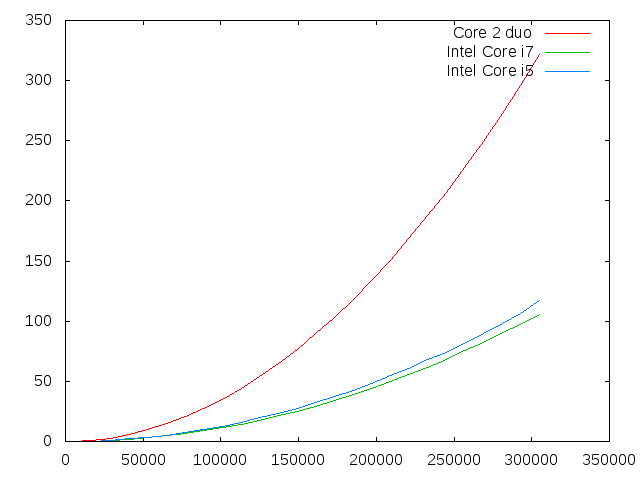
\includegraphics[width=1\textwidth]{insercion_dtos_pcs.png}
					\caption{Gráfica con tiempos de ejecución del algoritmo de Inserción en tres procesadores. Intel® Core™ i7-5500U CPU @ 2.40GHz, Intel® Core™ i5-2320 CPU @ 3.00GHz, Intel® Core™ 2 Duo T2350 @ 1.86GHz.}

				\end{figure}

				\par
				Como se puede observar, los tiempos varían de forma nada despreciable; es claro, sobre todo, el salto de velocidad entre el Intel Core 2 Duo y los otros dos debido a la distancia temporal y tecnológica entre ellos. Sin embargo, lo único que conseguimos es cambiar las constantes ocultas, por lo que generalmente es preferible buscar un algoritmo con un orden un poco mejor a costa de usar un hardware menos potente.

\newpage

			\subsubsection{Algoritmos del mismo orden en distintos procesadores.}

				\par
				Por otra parte, queremos observar qué ocurre si ejecutamos un algoritmo lento de un determinado orden de eficiencia en un procesador potente y un algoritmo rápido de ese mismo orden en un procesador poco potente. Como muestras tomaremos los algoritmos \textit{Burbuja} (lento) y de Inserción (rápido), correspondientes a un O($n^2$): 

				\begin{figure}[h]

					\centering
					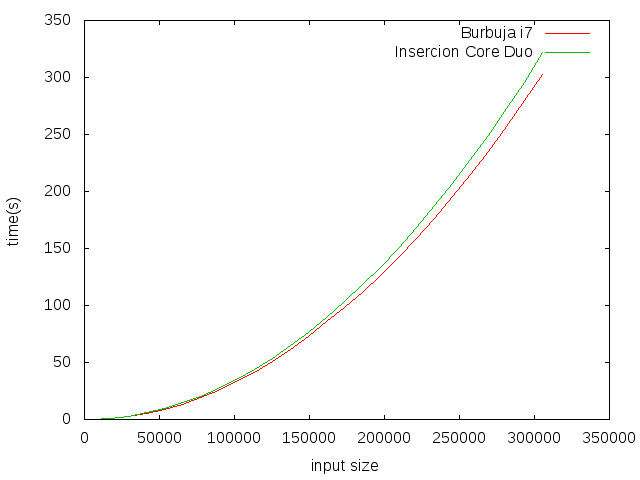
\includegraphics[width=1\textwidth]{burbuja_vs_insercion.png}
					\caption{Gráfica con tiempos de ejecución de los algoritmos \textit{Burbuja} e Inserción. Intel® Core™ i7-5500U CPU @ 2.40GHz, Intel® Core™ 2 Duo T2350 @ 1.86GHz.}

				\end{figure}

				\par
				En la comparativa de algoritmos de orden O($n^2$) veíamos que, bajo las mismas condiciones, el algoritmo \textit{Burbuja} es claramente más ineficiente que el de Inserción. Sin embargo, empleando hardware de muy distintas capacidades, podemos conseguir que el algoritmo \textit{Burbuja} gane al de Inserción; no obstante, entre la salida al mercado de cada uno de los dos procesadores comparados hay aproximadamente 10 años, lo cual dice mucho nuevamente acerca de la importancia de la eficiencia, incluso dentro del mismo orden, a la hora de tomar una decisión.

\newpage

			\par
			Para mayor claridad, adjuntamos la tabla de tiempos:

			\begin{figure}[h]

				\centering

				\begin{tabular}{| >{\centering\arraybackslash}m{1in} | >{\centering\arraybackslash}m{1in} | >{\centering\arraybackslash}m{1in} | >{\centering\arraybackslash}m{1in} |}

					\hline
					\textbf{Tamaño de $n$} & \textbf{Core 2 Duo ($s$)} & \textbf{Core i5 ($s$)} & \textbf{Core i7 ($s$)} \\
					\hline
					5000 & 0.092425 & 0.031133 & 0.02864 \\
					\hline
					17000 & 0.994135 & 0.364622 & 0.331283 \\
					\hline
					29000 & 2.90596 & 1.04985 & 0.95447 \\
					\hline
					41000 & 5.819 & 2.10168 & 1.98294 \\
					\hline
					53000 & 9.72427 & 3.49405 & 3.33574 \\
					\hline
					65000 & 14.6285 & 5.24682 & 5.05818 \\
					\hline
					77000 & 20.5247 & 7.36656 & 6.77307 \\
					\hline
					89000 & 27.3593 & 9.88673 & 9.02627 \\
					\hline
					101000 & 35.2544 & 12.5851 & 11.6468 \\
					\hline
					113000 & 44.1562 & 15.7986 & 14.5133 \\
					\hline
					125000 & 53.8809 & 19.978 & 17.7904 \\
					\hline
					137000 & 64.7697 & 23.2261 & 21.4265 \\
					\hline
					149000 & 76.4518 & 27.5321 & 25.2194 \\
					\hline
					161000 & 89.8139 & 32.2 & 29.4826 \\
					\hline
					173000 & 103.434 & 37.4744 & 34.036 \\
					\hline
					185000 & 118.276 & 42.5004 & 38.9165 \\
					\hline
					197000 & 133.757 & 48.0315 & 44.2132 \\
					\hline
					209000 & 150.313 & 54.6543 & 49.7696 \\
					\hline
					221000 & 168.566 & 60.7121 & 55.6643 \\
					\hline
					233000 & 187.793 & 68.1661 & 61.8095 \\
					\hline
					245000 & 206.859 & 74.2389 & 68.3384 \\
					\hline
					257000 & 227.995 & 81.7298 & 75.2418 \\
					\hline
					269000 & 249.363 & 89.945 & 82.2099 \\
					\hline
					281000 & 272.411 & 98.2273 & 90.579 \\
					\hline
					293000 & 295.85 & 106.383 & 97.4804 \\
					\hline
					305000 & 322.121 & 117.112 & 105.925 \\
					\hline

				\end{tabular}

			\end{figure}

\newpage

		\subsection{Sistema operativo.}

			\par
			Al igual que con distintas optimizaciones o distinto hardware, podríamos pensar que diferentes sistemas operativos harán nuestros algoritmos más lentos o más rápidos. En este apartado tratamos de dar respuesta a esa cuestión probando el algoritmo de Inserción en dos sistemas operativos.

			\begin{figure}[h]

				\centering
				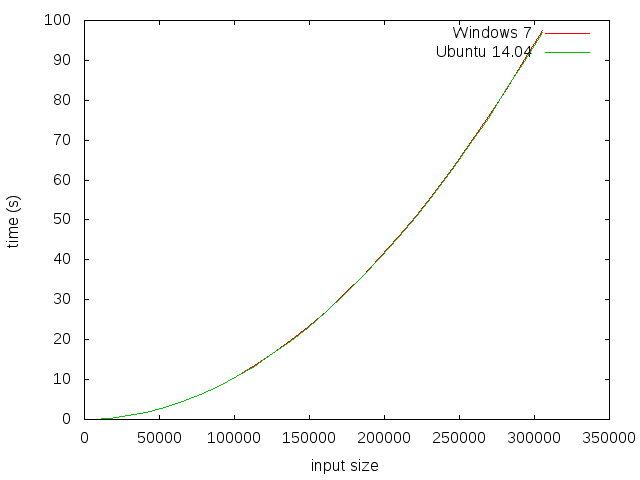
\includegraphics[width=1\textwidth]{insercion_2so.png}
				\caption{Gráfica con tiempos de ejecución del algoritmo de Inserción en dos sistemas operativos distintos: Ubuntu 14.04 y Windows 7. Intel® Core™ i5-3470 CPU @ 3.20GHz.}

			\end{figure}

			\par
			De aquí se extrae que, al menos en esta prueba, las diferencias observadas no son suficientes para poder afirmar que el rendimiento cambia de un sistema operativo a otro; Windows 7 parece ser ligeramente más lento conforme aumentamos el tamaño de la entrada del algoritmo, pero apenas se nota.

\newpage

			\par
			Para mayor claridad, adjuntamos la tabla de tiempos:

			\begin{figure}[h]

				\centering

				\begin{tabular}{| >{\centering\arraybackslash}m{1in} | >{\centering\arraybackslash}m{1in} | >{\centering\arraybackslash}m{1in} |}

					\hline
					\textbf{Tamaño de $n$} & \textbf{Tiempo Ubuntu 14.04 ($s$)} & \textbf{Tiempo Windows 7 ($s$)} \\
					\hline
					5000 & 0.029967 & 0.031 \\
					\hline
					17000 & 0.303031 & 0.312 \\
					\hline
					29000 & 0.883463 & 0.906 \\
					\hline
					41000 & 1.76988 & 1.779 \\
					\hline
					53000 & 2.952 & 2.948 \\
					\hline
					65000 & 4.45062 & 4.448 \\
					\hline
					77000 & 6.20768 & 6.24 \\
					\hline
					89000 & 8.29843 & 8.348 \\
					\hline
					101000 & 10.6655 & 10.697 \\
					\hline
					113000 & 13.3013 & 13.437 \\
					\hline
					125000 & 16.4174 & 16.417 \\
					\hline
					137000 & 19.6679 & 19.721 \\
					\hline
					149000 & 23.176 & 23.312 \\
					\hline
					161000 & 27.1208 & 27.167 \\
					\hline
					173000 & 31.271 & 31.477 \\
					\hline
					185000 & 35.7505 & 35.922 \\
					\hline
					197000 & 40.5161 & 40.801 \\
					\hline
					209000 & 45.621 & 45.794 \\
					\hline
					221000 & 51.001 & 51.184 \\
					\hline
					233000 & 56.6762 & 56.847 \\
					\hline
					245000 & 62.722 & 63.025 \\
					\hline
					257000 & 69.054 & 69.375 \\
					\hline
					269000 & 75.3449 & 75.949 \\
					\hline
					281000 & 82.8552 & 82.769 \\
					\hline
					293000 & 89.6191 & 90.176 \\
					\hline
					305000 & 97.1005 & 97.467 \\
					\hline

				\end{tabular}

			\end{figure}

\newpage

	\section{Análisis de eficiencia erróneos.}

		\par
		Antes de concluir, veamos qué ocurre si ajustamos una función errónea a los resultados de la ejecución de un algoritmo. En particular, la siguiente gráfica muestra el intento de ajustar una función $f(x)$ $=$ $n\log_{}n$ a un algoritmo cuadrático como es el \textit{Burbuja}:

		\begin{figure}[h]

			\centering
			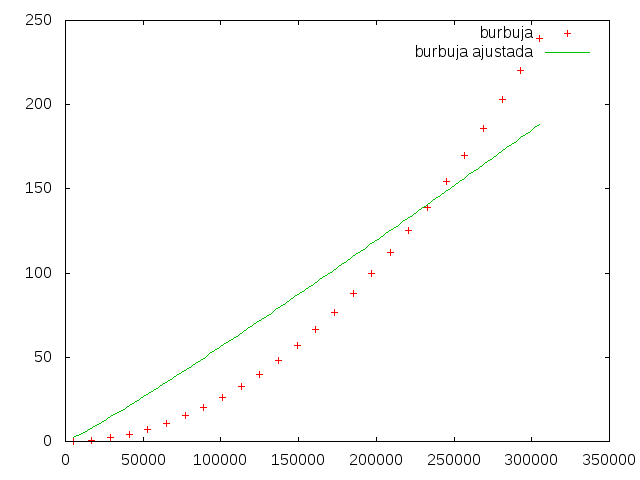
\includegraphics[width=1\textwidth]{burbuja_erroneo.png}
			\caption{Gráfica del algoritmo \textit{Burbuja} ajustada a $f(x)$. Compilación sin optimización. Intel® Core™ i7-5500U CPU @ 2.40GHz.}

		\end{figure}

		\par
		Se puede constatar que $f(x)$ difiere de la curva del algoritmo hasta tal punto que no podemos encontrar parecido. Con este ejemplo se aprecia bien la distinción entre órdenes de eficiencia.

\newpage

	\section{Conclusión.}

		\par
		Tras ver las diferentes comparaciones de tiempo entre todos estos algoritmos, podemos asegurar que el orden de eficiencia de un algoritmo no lo hará mejor a otro bajo cualquier circunstancia. Incluso puede resultar más eficiente un algoritmo de mayor orden para pequeñas cantidades de datos debido a las constantes ocultas. \\

		\par
		Otro de los hechos que hemos podido constatar es la diferencia entre los algoritmos que tienen el mismo orden de eficiencia. Centrándonos solo en la notación asintótica, se podría pensar que los algoritmos de ordenación por \textit{Burbuja}, Inserción o Selección son iguales a efectos de eficiencia; no obstante, si los estudiamos un poco más a fondo teniendo en cuenta sus constantes ocultas, veremos que existen grandes diferencias entre ellos. \\

		\par
		Para cerrar, diremos que la elección de los algoritmos basada en la eficiencia de los mismos y en las circunstancias de su uso es fundamental para obtener soluciones adecuadas y competitivas en términos de tiempo y de recursos hardware necesarios; en definitiva, mejores.

\end{document}